% EHMbrAIn — project presentation.
% Build:  latexmk -pdf -outdir=build EHMbrAIn-slides.tex   (from paper/slides/)
%
% Figures are the report's own auto-generated PDFs (norm N4): the slides never
% carry a number the pipeline did not produce.
%
% NOTE (public repository): the author remains anonymous in the repository.

\documentclass[aspectratio=169,10pt]{beamer}

\usetheme{metropolis}
\metroset{sectionpage=progressbar, numbering=fraction, progressbar=frametitle,
          block=fill}

\usepackage[utf8]{inputenc}
\usepackage[T1]{fontenc}
\usepackage{lmodern}
\usepackage[english]{babel}
\usepackage{amsmath,amssymb}
\usepackage{siunitx}
\usepackage{booktabs}
\usepackage{array}
\usepackage{graphicx}
\usepackage{tikz}
\usetikzlibrary{positioning,arrows.meta}
\usepackage{appendixnumberbeamer}
\graphicspath{{../report/figures/}}

% The report's auto-generated tables use \code; same definition here so the
% slides can \input them unchanged (norm N4).
\DeclareUrlCommand\code{\urlstyle{tt}\def\UrlBreaks{\do\/\do\_\do\.\do\-\do\:}}

% --- palette: the report's own ------------------------------------------
\definecolor{inkc}{HTML}{212529}
\definecolor{bluec}{HTML}{4263EB}
\definecolor{redc}{HTML}{A61E4D}
\definecolor{grayc}{HTML}{868E96}
\setbeamercolor{frametitle}{bg=inkc}
\setbeamercolor{progress bar}{fg=bluec}
\setbeamercolor{alerted text}{fg=redc}

\newcommand{\win}{\textcolor{bluec}{\textbf{AI}}}
\newcommand{\trad}{\textcolor{redc}{\textbf{traditional}}}
% one-line "what this slide says" strip, used on every content slide
\newcommand{\lead}[1]{{\footnotesize\itshape\color{grayc}#1}\par\smallskip}

\title{\textbf{EHMbrAIn}}
\subtitle{AI-based versus traditional engine health monitoring:\\
a gas path analysis testbed on the CFM56-7B with synthetic ground truth}
\date{\today}
\author{--- anonymous in the public repository ---}

\begin{document}

\maketitle

\begin{frame}[t]{Where this talk goes}
  \lead{Two levels throughout: what the result is, then the mechanism that produces it.}
  \tableofcontents
\end{frame}

% =========================================================================
\section{The problem}
% =========================================================================

\begin{frame}[t]{An engine degrades where nobody can look}
  \lead{The whole discipline exists because the interesting state is unobservable.}
  \begin{columns}[T]
    \begin{column}{0.56\textwidth}
      A commercial turbofan stays on the wing for years. Meanwhile:
      \begin{itemize}
        \item dust and pollution foul the compressors,
        \item hot-section parts creep and oxidize,
        \item tip clearances open, seals wear.
      \end{itemize}
      \medskip
      Nobody sees any of it. The airline sees \alert{a handful of numbers per
      flight}: shaft speeds, exhaust temperature, fuel flow.
      \medskip

      The stakes: a shop visit costs millions; an unscheduled removal disrupts a
      whole fleet schedule.
    \end{column}
    \begin{column}{0.44\textwidth}
      \centering
      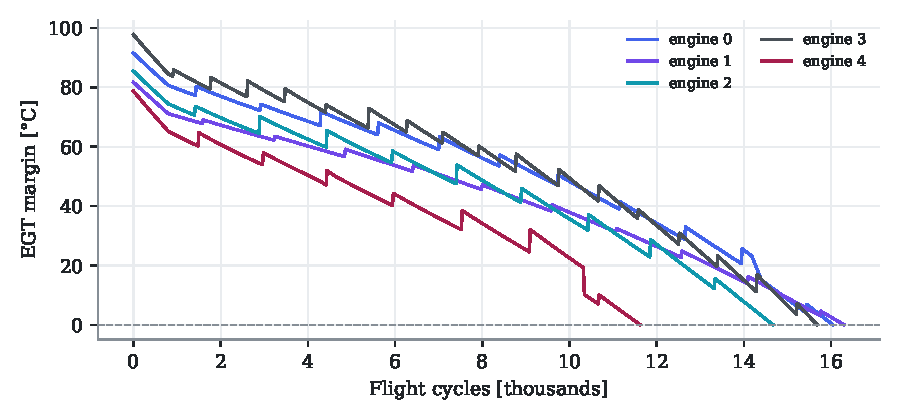
\includegraphics[width=\linewidth]{egtm_sawtooth}\\[-1mm]
      {\scriptsize The one aggregate an operator watches: exhaust-gas-temperature
      margin. Sawteeth are compressor washes; zero is retirement.}
    \end{column}
  \end{columns}
\end{frame}

\begin{frame}[t]{Two schools, and a broken comparison}
  \lead{The literature's structural weakness is the reason this project exists.}
  \begin{columns}[T]
    \begin{column}{0.48\textwidth}
      \textbf{\textcolor{redc}{Traditional EHM}} --- since the 1970s\\[2mm]
      Gas path analysis: invert a thermodynamic model to ask \emph{which
      component} degraded and \emph{by how much}. Around it: baselines, trend
      smoothing, Kalman filters, expert rules.
    \end{column}
    \begin{column}{0.48\textwidth}
      \textbf{\textcolor{bluec}{AI-based EHM}} --- last decade\\[2mm]
      Striking results on remaining-life prediction, mostly on synthetic
      benchmarks (C-MAPSS and successors).
    \end{column}
  \end{columns}
  \vspace{4mm}
  \begin{alertblock}{The gap}
    AI is almost never compared against a traditional pipeline \emph{implemented
    with equal care}, on the same data, with the same metrics and the same tuning
    effort. A stream of comparisons against straw men tells us nothing about what
    AI actually contributes, when, or at what cost.
  \end{alertblock}
\end{frame}

\begin{frame}[t]{What this project builds}
  \lead{A level playing field, plus the one thing no real fleet can provide.}
  \begin{enumerate}
    \item A \textbf{calibrated thermodynamic twin} of the CFM56-7B26, built only
      from certified public data.
    \item \textbf{SynCFM56}: 100 virtual engines run to failure, in airline
      snapshot format, carrying \alert{complete ground truth} --- the true health
      of every component at every flight.
    \item Both EHM families on \emph{identical} data, metrics, splits and tuning
      budget, adjudicated under a \textbf{pre-registered protocol}.
  \end{enumerate}
  \vspace{3mm}
  \begin{block}{Why ground truth changes the question}
    On a real fleet you can ask ``did the method predict well?''. Only with
    synthetic truth can you ask \alert{``did it blame the right component?''} ---
    which is exactly where traditional GPA is weakest and AI is least transparent.
  \end{block}
\end{frame}

% =========================================================================
\section{The physics, and why diagnosis is hard}
% =========================================================================

\begin{frame}[t]{The machine, in one picture}
  \lead{Two independent spools; the station numbers every later slide uses.}
  \centering
  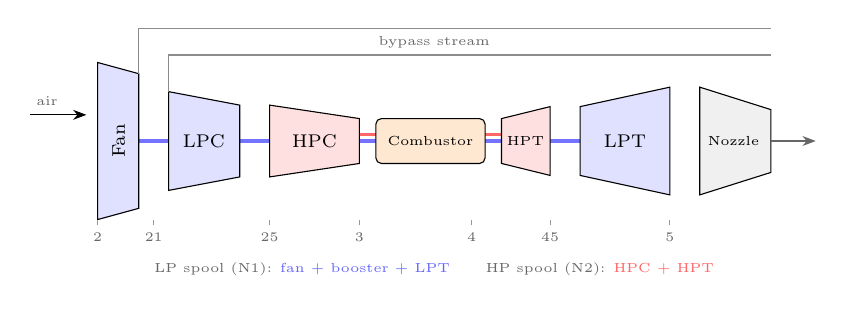
\begin{tikzpicture}[scale=0.95, every node/.style={transform shape},
      font=\scriptsize, st/.style={font=\tiny, text=black!60}]
    \draw[blue!55, line width=1.6pt] (0.05,0) -- (7.65,0);
    \draw[red!60, line width=1.0pt] (2.35,0.09) -- (6.05,0.09);
    \draw[fill=blue!12] (0,-1.05) -- (0,1.05) -- (0.55,0.9) -- (0.55,-0.9) -- cycle;
    \node[rotate=90] at (0.28,0.0) {Fan};
    \draw[fill=blue!12] (0.95,-0.66) -- (0.95,0.66) -- (1.9,0.48) -- (1.9,-0.48) -- cycle;
    \node at (1.42,0) {LPC};
    \draw[fill=red!12] (2.3,-0.48) -- (2.3,0.48) -- (3.5,0.3) -- (3.5,-0.3) -- cycle;
    \node at (2.9,0) {HPC};
    \draw[fill=orange!18, rounded corners=2pt] (3.72,-0.3) rectangle (5.18,0.3);
    \node[font=\tiny] at (4.45,0) {Combustor};
    \draw[fill=red!12] (5.4,-0.3) -- (5.4,0.3) -- (6.05,0.46) -- (6.05,-0.46) -- cycle;
    \node[font=\tiny] at (5.72,0) {HPT};
    \draw[fill=blue!12] (6.45,-0.46) -- (6.45,0.46) -- (7.65,0.72) -- (7.65,-0.72) -- cycle;
    \node at (7.05,0) {LPT};
    \draw[fill=black!6] (8.05,-0.72) -- (8.05,0.72) -- (9.0,0.42) -- (9.0,-0.42) -- cycle;
    \node[font=\tiny] at (8.5,0) {Nozzle};
    \draw[black!45] (0.55,0.9) -- (0.55,1.5) -- (9.0,1.5);
    \draw[black!45] (0.95,0.66) -- (0.95,1.15) -- (9.0,1.15);
    \node[st] at (4.5,1.32) {bypass stream};
    \draw[-{Stealth}] (-0.9,0.35) -- (-0.15,0.35) node[pos=0.3, above, st] {air};
    \draw[-{Stealth}, black!60] (9.0,0) -- (9.6,0);
    \foreach \x/\lbl in {0/2, 0.75/21, 2.3/25, 3.5/3, 5.0/4, 6.05/45, 7.65/5}{
      \draw[black!40] (\x,-1.05) -- (\x,-1.12);
      \node[st] at (\x,-1.28) {\lbl};}
    \node[st, align=center] at (4.5,-1.72)
      {LP spool (N1): \textcolor{blue!60}{fan + booster + LPT}\qquad
       HP spool (N2): \textcolor{red!60}{HPC + HPT}};
  \end{tikzpicture}
  \vspace{2mm}

  {\small The airline receives \alert{N1, N2, EGT and fuel flow} --- the ``cockpit
  set''. Optional packages add pressures and temperatures at stations 25 and 3.}
\end{frame}

\begin{frame}[t]{Gas path analysis: the model to invert}
  \lead{Ten unknowns, three usable measurements. That ratio is the whole story.}
  \textbf{Health state} --- two numbers per turbomachine, in \% off a new engine:
  \[
    \mathbf{x} = [\Delta\eta_{\mathrm{fan}}, \Delta\Gamma_{\mathrm{fan}},
    \ldots, \Delta\eta_{\mathrm{LPT}}, \Delta\Gamma_{\mathrm{LPT}}]^{\mathsf T}
    \in \mathbb{R}^{10}
  \]
  $\eta$: isentropic efficiency (dirt and wear reduce it). $\Gamma$: flow
  capacity (fouling closes compressors; erosion opens turbines).
  \medskip

  \textbf{What is measurable} --- deviations from a healthy-engine baseline:
  \[
    \Delta\mathbf{z} \;=\; \underbrace{\mathbf{H}(\mathbf{u})}_{\text{influence matrix}}\mathbf{x}
    \;+\; \mathbf{S}\mathbf{b} \;+\; \mathbf{v},
    \qquad \mathbf{v}\sim\mathcal{N}(\mathbf{0},\mathbf{R})
  \]
  \medskip

  \begin{alertblock}{The inversion is ill-posed}
    With the cockpit set, $\operatorname{rank}(\mathbf{H}) = 3$ for 10 unknowns.
    Infinitely many health states explain the same measurements. Regularized
    weighted least squares picks one --- and pays for it in bias.
  \end{alertblock}
\end{frame}

\begin{frame}[t]{Smearing: how a diagnosis flips to the wrong component}
  \lead{Two faults, two measurements, one noise-sized error. Nothing here is a bug.}
  \begin{columns}[T]
    \begin{column}{0.5\textwidth}
      Two health parameters, two channels:
      $\mathbf{H} = \left(\begin{smallmatrix} 1.0 & 0.9 \\ 0.5 & 0.5\end{smallmatrix}\right)$.
      \medskip

      Truth: HPC fault only, $\mathbf{x}=(-1,0)$. Exact measurements invert perfectly.
      \medskip

      Perturb one channel by $+0.1$ --- one noise standard deviation --- and the
      inversion returns $\hat{\mathbf{x}} = (0,-1)$:
      \medskip

      \alert{HPC healthy, HPT degraded.} The information is not in the measurements
      when two signatures nearly coincide.
    \end{column}
    \begin{column}{0.5\textwidth}
      \centering
      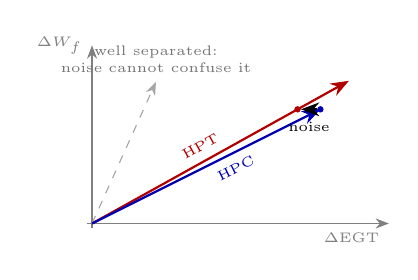
\begin{tikzpicture}[scale=2.9, font=\scriptsize, >={Stealth}]
        \draw[->, black!50] (-0.02,0) -- (1.30,0) node[below left, font=\tiny] {$\Delta$EGT};
        \draw[->, black!50] (0,-0.02) -- (0,0.78) node[left, font=\tiny] {$\Delta W_f$};
        \draw[->, black!35, dashed] (0,0) -- (0.28,0.62)
          node[above, font=\tiny, align=center, text=black!55] {well separated:\\noise cannot confuse it};
        \draw[->, thick, red!70!black] (0,0) -- (1.125,0.625)
          node[pos=0.45, above=0pt, sloped, font=\tiny] {HPT};
        \draw[->, thick, blue!70!black] (0,0) -- (1.0,0.5)
          node[pos=0.6, below=0pt, sloped, font=\tiny] {HPC};
        \fill[blue!70!black] (1.0,0.5) circle (0.014);
        \draw[->, black, thick] (0.985,0.5) -- (0.915,0.5) node[midway, below=1pt, font=\tiny] {noise};
        \fill[red!70!black] (0.9,0.5) circle (0.014);
      \end{tikzpicture}\\[1mm]
      {\scriptsize The two fault signatures sit $2.5^{\circ}$ apart. One nudge moves
      the reading from one ray onto the other.}
    \end{column}
  \end{columns}
\end{frame}

\begin{frame}[t]{This engine's actual geometry}
  \lead{The wall is not hypothetical: it is measured, and it does not move.}
  \begin{columns}[T]
    \begin{column}{0.55\textwidth}
      \centering
      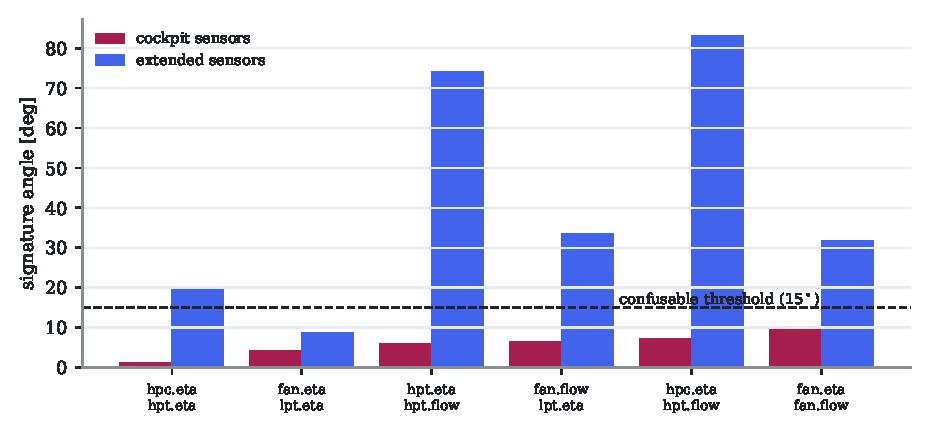
\includegraphics[width=\linewidth]{confusable_angles}
    \end{column}
    \begin{column}{0.45\textwidth}
      With the \textbf{cockpit set}:
      \begin{itemize}\small
        \item minimum signature angle \alert{$1.3^{\circ}$}
          ($\eta_{\mathrm{HPC}}$ vs $\eta_{\mathrm{HPT}}$),
        \item seven pairs below $15^{\circ}$,
        \item rank 3 of 10.
      \end{itemize}
      \medskip
      With the \textbf{extended set} (P25/T25/PS3/T3): rank 7, minimum angle
      $\times 5$.
      \medskip

      Repeated over a six-point envelope grid, the structure barely moves
      ($1.2$--$1.4^{\circ}$): \alert{the blindness is intrinsic to the sensor set},
      not to one flight condition.
    \end{column}
  \end{columns}
\end{frame}

% =========================================================================
\section{The testbed}
% =========================================================================

\begin{frame}[t]{The twin: certified data in, predictions out}
  \lead{Calibrated against measurements it was never fitted to --- that is the test.}
  \begin{columns}[T]
    \begin{column}{0.52\textwidth}
      Built in pyCycle by morphing a validated NASA example, \alert{at most three
      parameters per step}, convergence required at each.
      \medskip

      Calibration uses only \textbf{measured certified data}: type-certificate
      limits, and the ICAO databank's sea-level test-bed \emph{fuel flows}.
      \medskip

      Points are solved \emph{thrust-matched}, so the model's fuel flow is a
      \alert{prediction} confronted with the measurement --- not a fitted quantity.
      \medskip

      Result: takeoff $-1.4\,\%$, climb-out $-2.2\,\%$, approach $-3.1\,\%$.
      Cruise TSFC lands within $2\,\%$ of the published value \emph{without being
      a target}.
    \end{column}
    \begin{column}{0.48\textwidth}
      \centering
      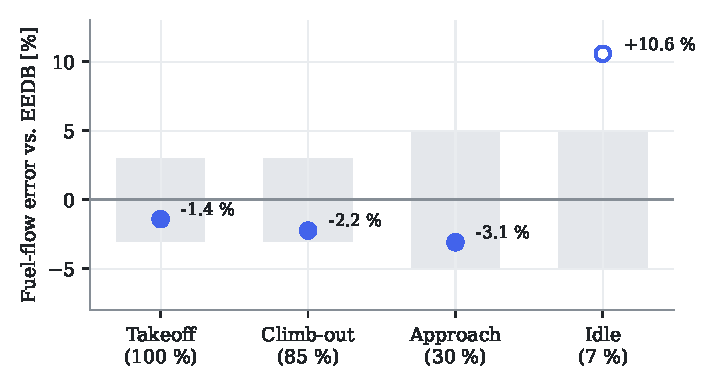
\includegraphics[width=\linewidth]{anchor_errors}\\[-1mm]
      {\scriptsize Gray bands are the contract tolerances, fixed \emph{before}
      the run. The hollow marker (idle) is reported but not gated --- deep
      part power is generic-map territory.}
    \end{column}
  \end{columns}
\end{frame}

\begin{frame}[t]{The fleet: six mechanisms, one hundred lives}
  \lead{Each mechanism is a closed-form function of flight cycle, stored separately.}
  \centering
  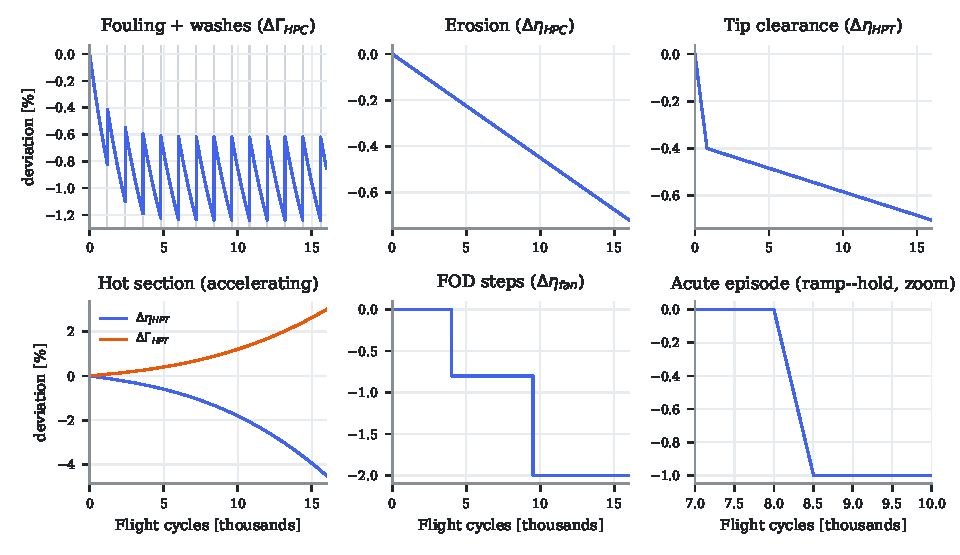
\includegraphics[width=0.70\textwidth]{degradation_profiles}\\[1mm]
  {\scriptsize Drawn by the generator's own code. Each contribution is stored apart, so the
  fleet records not just \emph{how} degraded an engine is but \alert{\emph{by what}}.}
\end{frame}

\begin{frame}[t]{Making the benchmark hard on purpose}
  \lead{A synthetic dataset's commonest disease is being accidentally easy.}
  \begin{block}{The difficulty gate}
    A deliberately weak classifier (logistic regression on raw channels) must
    \emph{fail} to solve the isolation task. Threshold set in advance: $60\,\%$.
  \end{block}
  \vspace{2mm}
  \begin{columns}[T]
    \begin{column}{0.5\textwidth}
      \textbf{First pass: failed at $81.6\,\%$.}\\[1mm]
      Root cause: chronic mechanisms co-evolve with age, so the label was an
      \alert{age proxy}, not a fault label. The task was never isolation.
      \medskip

      Fix was \emph{structural}, not cosmetic: discrete single-parameter acute
      fault episodes, drawn from the confusable pairs.
    \end{column}
    \begin{column}{0.5\textwidth}
      \textbf{Second pass: $54.0\,\%$ --- pass.}\\[1mm]
      And on fleet v1.1 the gate bit \alert{again} ($62.2\,\%$): fault magnitudes
      were scaled by $0.75$ until it passed at $58.1\,\%$.
      \medskip

      An audit also caught a generator bug: episode onsets drawn against the
      simulation horizon instead of engine life.
    \end{column}
  \end{columns}
  \vspace{2mm}
  {\small Both failures are in the report in full. A gate that cannot fail
  certifies nothing.}
\end{frame}

\begin{frame}[t]{Four safeguards, fixed before any contestant ran}
  \lead{The comparison is itself an instrument, and it was designed first.}
  \begin{columns}[T]
    \begin{column}{0.5\textwidth}
      \textbf{Pre-registration.} Hypotheses, thresholds, splits (with file
      hashes), tests and stopping rule frozen under a git tag before the
      confirmatory run.
      \medskip

      \textbf{Symmetric tuning.} 50 Optuna trials \emph{each}. The comparison is
      between two tuned practitioners, not a tuned one and a default one.
    \end{column}
    \begin{column}{0.5\textwidth}
      \textbf{Split by engine}, 70/10/20, never by flight --- flights of one
      engine are near-duplicates. Leakage checked in CI.
      \medskip

      \textbf{A strong baseline.} The traditional pipeline is built to industrial
      shape, every expert rule justified; smearing is \emph{measured} against
      truth, not assumed.
    \end{column}
  \end{columns}
  \vspace{3mm}
  \begin{alertblock}{Evidence hierarchy}
    Numbers exist in two castes and are never mixed: \emph{exploratory} (produced
    while building) and \emph{confirmatory} (produced once, after the freeze, on
    data touched exactly once). Only the second supports a verdict.
  \end{alertblock}
\end{frame}

% =========================================================================
\section{What classical GPA delivers here}
% =========================================================================

\begin{frame}[t]{The experiment: honest forward, classical inverse}
  \lead{Inverting the matrix that generated the data would be circular.}
  \begin{columns}[T]
    \begin{column}{0.5\textwidth}
      \textbf{Forward (plays the engine)}\\
      The \alert{nonlinear} neural twin: full physics curvature,
      $13$--$19\times$ closer to pyCycle than a linearization.
      \medskip

      \textbf{Inverse (plays the monitoring system)}\\
      The \alert{linear} regularized WLS on the influence matrix, at registered
      defaults --- and, like every fielded GPA, unaware the physics is curved.
    \end{column}
    \begin{column}{0.5\textwidth}
      \textbf{One run, end to end}\\[1mm]
      HPC loses $1\,\%$ efficiency. The cockpit sees N2 $-0.12\,\%$,
      $W_f$ $+0.57\,\%$, EGT $+0.52\,\%$.
      \medskip

      The inversion returns \alert{$-0.26\,\%$} on HPC efficiency --- a quarter of
      the truth --- and scatters the rest.
      \medskip

      Over 500 noise draws it names the HPC correctly \alert{$22\,\%$} of the
      time. Favourite wrong answer: the HPT.
    \end{column}
  \end{columns}
\end{frame}

\begin{frame}[t]{What the inversion gives back}
  \lead{Recovery and smearing, per parameter, per sensor set.}
  \centering
  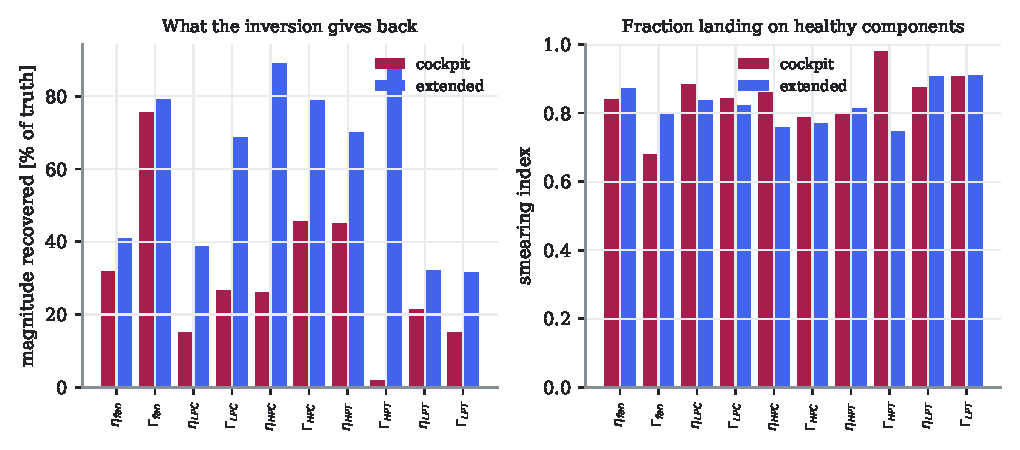
\includegraphics[width=0.78\textwidth]{gpa_recovery}\\[1mm]
  \begin{columns}[T]
    \begin{column}{0.48\textwidth}
      {\small Cockpit: \alert{$2$--$76\,\%$} recovered, median smearing
      \alert{$0.85$} --- six sevenths of the diagnosed magnitude lands on healthy
      components.}
    \end{column}
    \begin{column}{0.48\textwidth}
      {\small Extended: $32$--$90\,\%$, smearing barely moves ($0.82$). More
      sensors buy \emph{magnitude}, not tidiness.}
    \end{column}
  \end{columns}
\end{frame}

\begin{frame}[t]{How small a fault can be named}
  \lead{The practical resolution limit of each sensor package.}
  \centering
  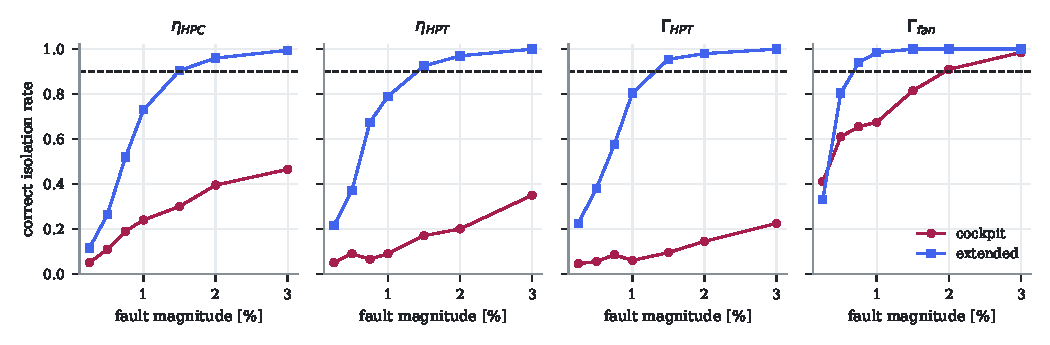
\includegraphics[width=0.82\textwidth]{gpa_detectability}\\[2mm]
  \begin{columns}[T]
    \begin{column}{0.46\textwidth}
      At the $90\,\%$-correct criterion, the cockpit set resolves
      \alert{one parameter of ten}; the extended set resolves \alert{seven},
      several from $0.75$--$1.5\,\%$.
    \end{column}
    \begin{column}{0.5\textwidth}
      The fleet's own faults are $0.3$--$1.1\,\%$. \alert{Most faults in this
      benchmark sit below the cockpit set's resolution limit} --- which is why the
      isolation contest later ends where it does.
    \end{column}
  \end{columns}
\end{frame}

\begin{frame}[t]{A real engine, eight faults at once}
  \lead{Single-fault studies are the exercise; this is the situation.}
  \centering
  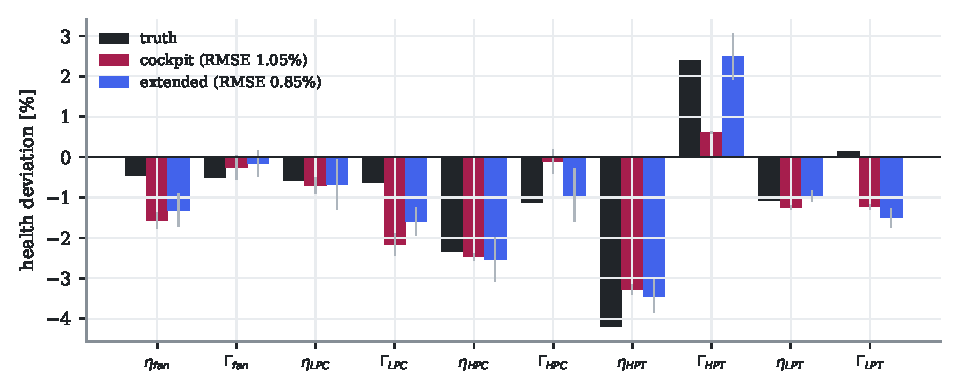
\includegraphics[width=0.72\textwidth]{gpa_multifault}\\[1mm]
  {\small True state: HPT efficiency $-4.2\,\%$ with flow capacity opened
  $+2.4\,\%$. The cockpit diagnosis gets the headline (HPT $-3.3$) but returns
  $+0.6$ for the flow opening --- \alert{the eroded-nozzle fingerprint is absent}.
  Both sets also \alert{invent} deterioration: fan efficiency three times its
  true value, LPT flow wrong in sign. A decision on those two numbers opens a
  healthy module.}
\end{frame}

% =========================================================================
\section{The pre-registered contest}
% =========================================================================

\begin{frame}[t]{Five hypotheses, one confirmatory pass}
  \lead{Three confirmed, two refuted. The split is the message.}
  \vspace{-1mm}
  \centering{\scriptsize% AUTOGENERATED by scripts/make_report_assets.py — do NOT edit by hand
\begin{tabular}{>{\raggedright\arraybackslash}p{0.16\textwidth}>{\raggedright\arraybackslash}p{0.15\textwidth}>{\raggedright\arraybackslash}p{0.41\textwidth}r}
\toprule
Hypothesis & Verdict & Confirmatory evidence (AI vs traditional) & $p$ (Holm) \\
\midrule
  H1 (detection) & CONFIRMED & recall 0.48 vs 0.13; delay 499 vs 6033 cy; FA 1=1 & 0.008 \\
  H2 (confusable isolation) & REFUTED & 0.31 vs 0.31 (n=13; discordant 4/4) & 0.64 \\
  H3 (RUL prognosis) & CONFIRMED & RMSE 1694/858 vs 3816/1981 cy (50/90\,\% life); $\delta$=0.89 & 8.6e-06 \\
  H4 (physics hybrid) & REFUTED & hybrid worse at 10/25/100\,\% (2852 vs 1772 cy at 10\,\%) & --- \\
  H5 (uncertainty) & CONFIRMED & coverage 0.883 vs 0.983 (nominal 0.90); half-width 1957 vs 11509 cy & --- \\
\bottomrule
\end{tabular}
}
  \vspace{3mm}

  {\small Both families tuned under the frozen 50-trial budget; the 20 test
  engines evaluated \alert{exactly once}; Wilcoxon paired by engine, one-sided
  exact McNemar for binary outcomes, Holm correction, BCa intervals.}
  \medskip

  {\small \alert{The two refutations did more work than the three confirmations:} H2 turned
  an algorithm question into a purchase order, H4 removed a popular technique from the
  shortlist.}
\end{frame}

\begin{frame}[t]{H1 --- the story is the tuning, not the model}
  \lead{An honest budget moved the answer; that is itself the finding.}
  \begin{columns}[T]
    \begin{column}{0.45\textwidth}
      \centering
      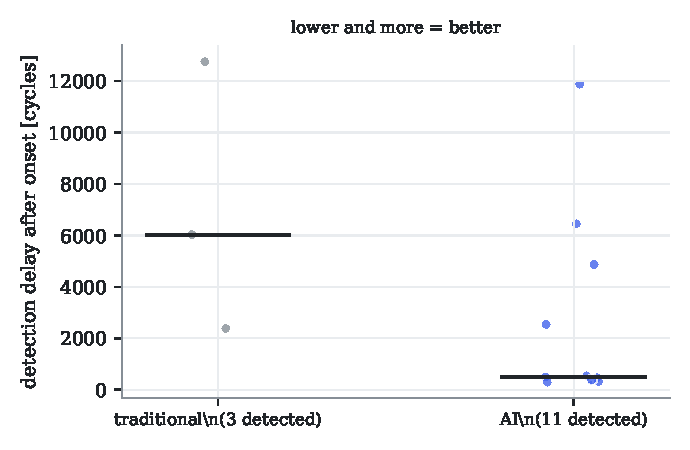
\includegraphics[width=0.86\linewidth]{detection_delays}
    \end{column}
    \begin{column}{0.55\textwidth}
      Untuned, the AI detector scored recall $0.06$ and the report called it
      ``a design gap, not a threshold gap''.
      \medskip

      The frozen search space contained the suspected lever --- \alert{feature
      window length}. Fifty trials stretched the windows: recall
      \alert{$0.48$} at a $499$-cycle median delay, twelve times earlier than
      the tuned classical detector, at equal false alarms.
      \medskip

      {\small Two transferable lessons: window length is the first knob any change
      detector lives or dies by; and threshold selection on small clean validation
      samples is fragile for \emph{any} method.}
    \end{column}
  \end{columns}
\end{frame}

\begin{frame}[t]{H2 refuted --- the wall binds everyone}
  \lead{Predicted by geometry before any model ran, and confirmed by both families.}
  \begin{columns}[T]
    \begin{column}{0.6\textwidth}
      \centering
      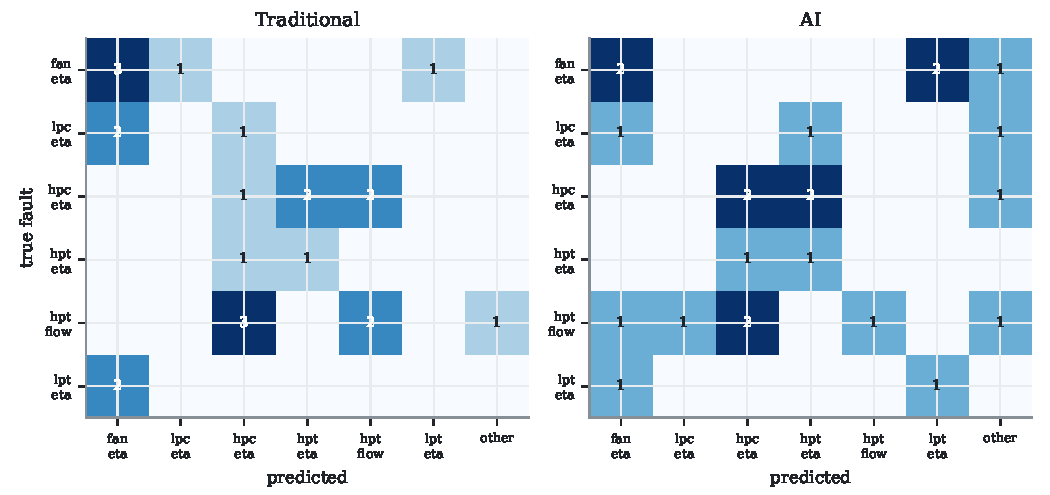
\includegraphics[width=\linewidth]{isolation_confusion}
    \end{column}
    \begin{column}{0.4\textwidth}
      On the thirteen confusable test episodes the families tie \alert{exactly}:
      $31\,\%$ each, with a perfectly symmetric disagreement pattern (four
      episodes only the AI gets, four only the rule gets).
      \medskip

      \begin{alertblock}{The conclusion is hardware}
        If confusable isolation matters operationally, \alert{add gas-path
        instrumentation}. No amount of modelling recovers information the sensors
        never captured.
      \end{alertblock}
    \end{column}
  \end{columns}
\end{frame}

\begin{frame}[t]{H3 and H5 --- prognosis is where learning pays}
  \lead{Not just a lower error: a differently shaped error.}
  \begin{columns}[T]
    \begin{column}{0.5\textwidth}
      \centering
      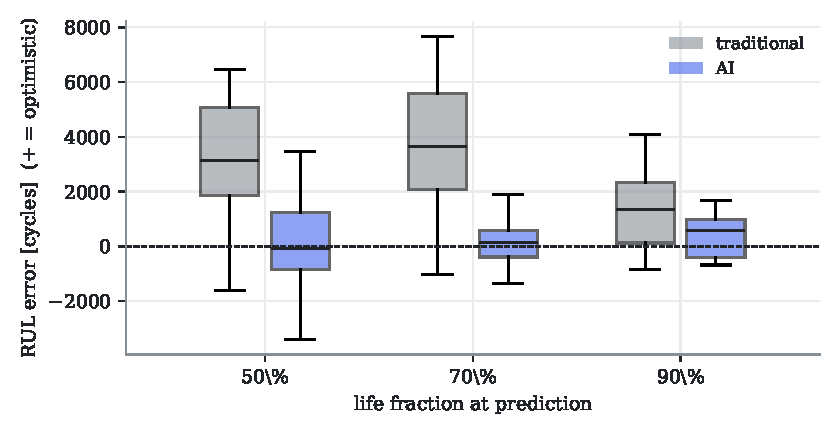
\includegraphics[width=0.98\linewidth]{rul_distribution}
    \end{column}
    \begin{column}{0.5\textwidth}
      RMSE \alert{$1694/1042/858$} cycles at $50/70/90\,\%$ of life, against
      $3816/4544/1981$. Cliff's $\delta = 0.89$, Holm $p = 8.6\times10^{-6}$.
      \medskip

      \textbf{Two scales, both true:} $\sim$2.3$\times$ over the extrapolation an operator
      fields \emph{today}, $\sim$1.3$\times$ over the best \emph{advanced} classical
      prognostic.
      \medskip

      Traditional errors are wide and \alert{skewed optimistic} --- the dangerous direction;
      the AI's are tight and near-unbiased.
      \medskip

      \textbf{H5}: conformal intervals \alert{six times narrower} than the slope band
      ($\pm1957$ vs $\pm11\,509$ cy) at honest coverage.
    \end{column}
  \end{columns}
\end{frame}

\begin{frame}[t]{H4 refuted --- physics features are not free wins}
  \lead{The popular default of concatenating estimator outputs is a documented negative.}
  \begin{columns}[T]
    \begin{column}{0.5\textwidth}
      \centering
      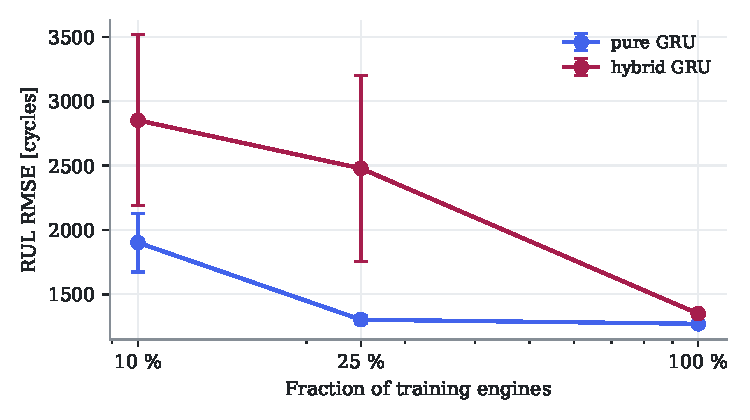
\includegraphics[width=0.95\linewidth]{hybrid_ablation}
    \end{column}
    \begin{column}{0.5\textwidth}
      Feeding the Kalman-tracked health parameters to the network alongside the
      raw deviations made it \alert{worse at every data fraction} --- and
      \emph{most} worse exactly where the hypothesis predicted it would help
      most.
      \medskip

      Mechanism, in hindsight: those estimates are heavily smeared. They add ten
      noisy, mutually correlated channels whose information is already present in
      the three deviations they were computed from.
      \medskip

      {\small Refuted a \alert{second, independent way} later, with twin-residual
      features on a nonlinear fleet.}
    \end{column}
  \end{columns}
\end{frame}

\begin{frame}[t]{Does the ranking survive outside our own simulator?}
  \lead{A benchmark this project had no hand in generating.}
  \begin{columns}[T]
    \begin{column}{0.55\textwidth}
      Re-ran the prognosis question on NASA's \textbf{C-MAPSS FD001}, the field's
      reference turbofan run-to-failure benchmark, with the same method shapes and
      three seeds.
      \medskip

      \begin{block}{Result}
        RMSE \alert{$14.9$} cycles (AI) versus \alert{$42.1$} (traditional) ---
        same direction, comparable magnitude of advantage, and an absolute figure
        competitive with published results.
      \end{block}
    \end{column}
    \begin{column}{0.45\textwidth}
      \textbf{Disclosed substitution}: the plan named N-CMAPSS, whose multi-gigabyte
      distribution breaks the project's desktop-reproducibility norm. FD001 answers
      the same ranking question at 5\,MB, and only prognosis transfers (FD001 has no
      event labels).
      \medskip

      {\small The prognosis conclusion is not an artifact of SynCFM56.}
    \end{column}
  \end{columns}
\end{frame}

% =========================================================================
\section{Beyond the wall}
% =========================================================================

\begin{frame}[t]{Can observability be bought without hardware?}
  \lead{The influence matrix changes with flight condition --- so the schedule is a design variable.}
  \begin{columns}[T]
    \begin{column}{0.52\textwidth}
      \centering
      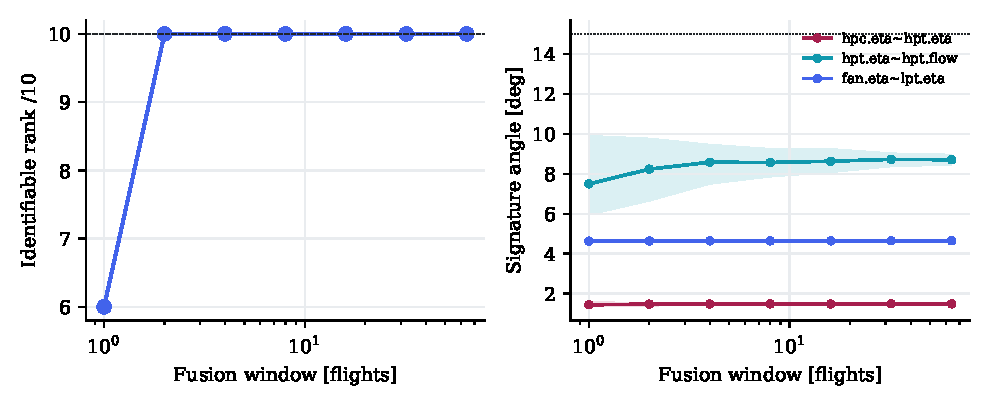
\includegraphics[width=\linewidth]{f7_observability}\\[-1mm]
      {\scriptsize Free ambient and power scatter restores algebraic rank
      immediately, but signature angles \alert{saturate}: free variation is real
      but thin.}
    \end{column}
    \begin{column}{0.48\textwidth}
      \textbf{Two cheaper exits than new probes:}
      \medskip

      \textbf{1. Redesign the report schedule.} One added periodic low-power
      cruise report buys \alert{$+79\,\%$} separability on the HPT ambiguity. The
      cost is a procedure bulletin, not avionics.
      \medskip

      \textbf{2. Learn the fusion, keep the physics.} A network fed per-flight
      \emph{physics inversions} isolates at $0.65$ against classical stacking's
      $0.17$; fed raw sequences instead, it fails outright at $0.12$.
      \medskip

      {\small What no schedule fixes: $\eta_{\mathrm{HPC}}\!\sim\!\eta_{\mathrm{HPT}}$
      stays below $1.8^{\circ}$ everywhere. That pair is \alert{fundamental}.}
    \end{column}
  \end{columns}
\end{frame}

\begin{frame}[t]{Only a real sensor breaks the wall}
  \lead{The data-processing inequality, made operational.}
  \begin{columns}[T]
    \begin{column}{0.42\textwidth}
      \centering
      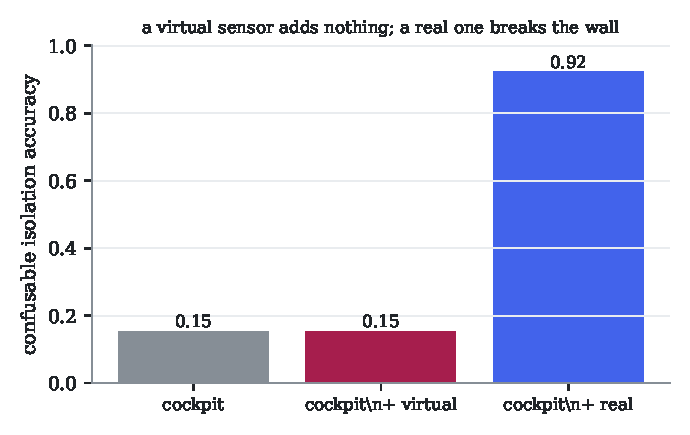
\includegraphics[width=0.92\linewidth]{wall_break}
    \end{column}
    \begin{column}{0.58\textwidth}
      Three sensor conditions on the confusable episodes:
      \begin{itemize}\small
        \item cockpit only: $0.15$
        \item cockpit $+$ \emph{model-predicted} station channels:
          \alert{$0.15$} ($p = 1.000$)
        \item cockpit $+$ \emph{real} station channels: \alert{$0.92$}
          ($p = 0.001$)
      \end{itemize}
      \medskip

      A quantity computed from the cockpit data cannot carry information the
      cockpit data did not hold. \alert{No software vendor can substitute a
      virtual sensor for a missing measurement.}
      \medskip

      {\small Cheap in practice: PS3, T25 and T3 are already measured by the FADEC
      for control. The barrier is recording and downlinking them, not new
      hardware.}
    \end{column}
  \end{columns}
\end{frame}

\begin{frame}[t]{A certificate of what a diagnosis can know}
  \lead{And --- uniquely --- a proof that the certificate is honest.}
  \begin{columns}[T]
    \begin{column}{0.56\textwidth}
      \centering
      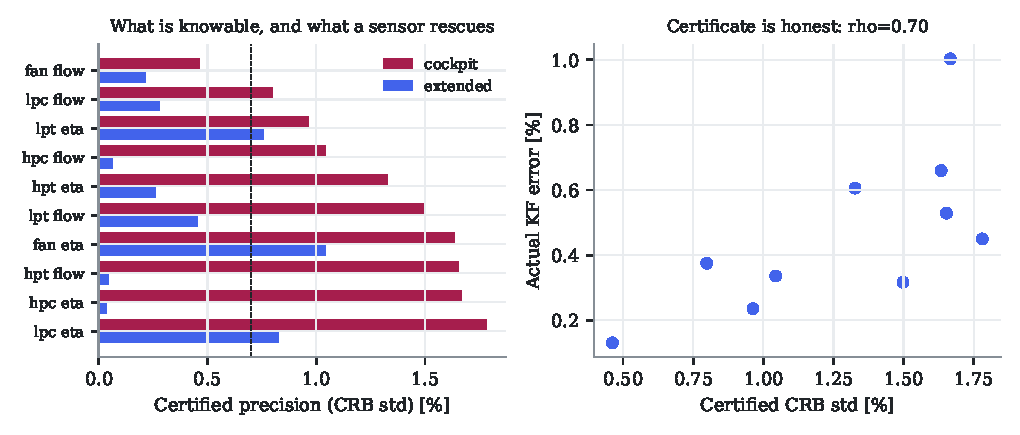
\includegraphics[width=\linewidth]{f10_certificate}
    \end{column}
    \begin{column}{0.44\textwidth}
      Accumulate Fisher information over an engine's \emph{own} flown conditions:
      \[
        \mathbf{F} = \mathbf{P}_0^{-1} + \textstyle\sum_t \mathbf{H}(u_t)^{\!\top}\mathbf{R}^{-1}\mathbf{H}(u_t)
      \]
      The Cram\'er--Rao bound $\mathbf{F}^{-1}$ states the best per-direction
      precision \emph{any} unbiased estimator can reach from this engine's data.
      \medskip

      \textbf{The proof} (right panel): certified precision ranks the filter's
      \emph{actual} error against ground truth, \alert{$\rho = 0.70$}, $p = 0.025$ ---
      the validation only a synthetic-truth benchmark can perform.
    \end{column}
  \end{columns}
\end{frame}

\begin{frame}[t]{Is a large RUL error the method's fault, or the future's?}
  \lead{Different problems, opposite remedies. Confusing them wastes budget.}
  \begin{columns}[T]
    \begin{column}{0.5\textwidth}
      \centering
      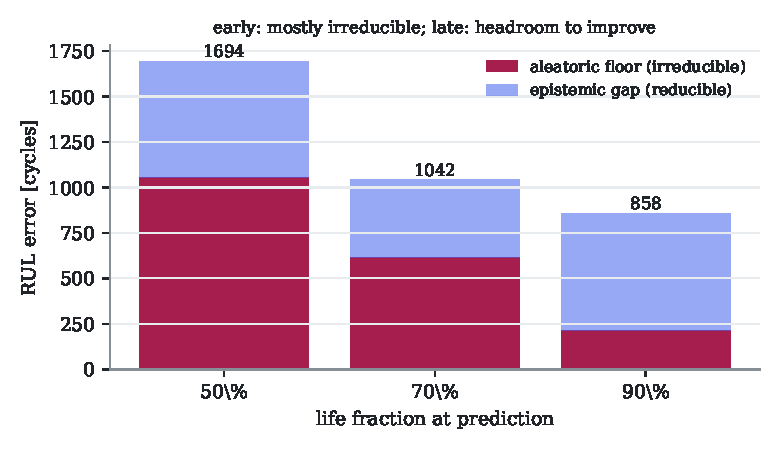
\includegraphics[width=\linewidth]{prognostic_floor}
    \end{column}
    \begin{column}{0.5\textwidth}
      Condition on each engine's \emph{true} current health, find its nearest
      neighbours in health space, and measure the spread of their \emph{true}
      remaining lives. Two engines in the same state that fail hundreds of cycles
      apart differ for reasons no present measurement contains.
      \medskip

      \textbf{At mid-life}: $87\,\%$ of the RUL spread is \alert{irreducible}.
      Remaining life is, to first order, not written in the present.
      \medskip

      \textbf{Late in life}: a \alert{$4\times$} reducible gap opens. That is
      where a better prognostic is worth building --- and only there.
    \end{column}
  \end{columns}
\end{frame}

\begin{frame}[t]{The determinability map: when does each approach win?}
  \lead{Sensor quality changes who wins; sensor placement changes what is knowable.}
  \centering
  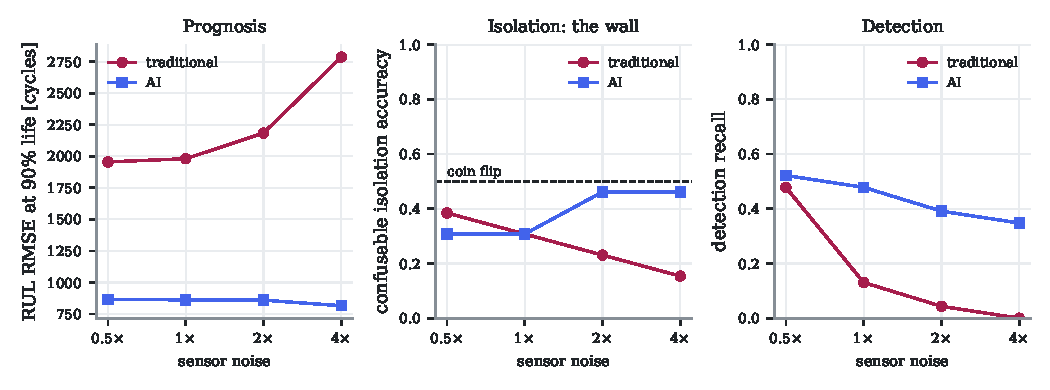
\includegraphics[width=0.82\textwidth]{noise_sweep}\\[1mm]
  \begin{columns}[T]
    \begin{column}{0.32\textwidth}
      {\scriptsize \textbf{Prognosis is noise-proof.} The AI's error is flat
      across a factor of eight in noise; the advantage \alert{widens} from
      $2.3\times$ to $3.4\times$.}
    \end{column}
    \begin{column}{0.32\textwidth}
      {\scriptsize \textbf{The wall is geometric.} Halving every $\sigma$ leaves
      confusable isolation at $0.31$--$0.38$. \alert{Buy new stations, not better
      probes at the old ones.}}
    \end{column}
    \begin{column}{0.32\textwidth}
      {\scriptsize \textbf{Thresholds fall off a cliff.} Classical detection goes
      from $0.48$ recall to zero; the AI holds $0.35$ at quadruple noise.}
    \end{column}
  \end{columns}
\end{frame}

\begin{frame}[t]{What it is worth --- and why it might be nothing}
  \lead{One mechanism monetized, because it is the only one the results support.}
  \begin{columns}[T]
    \begin{column}{0.5\textwidth}
      \centering
      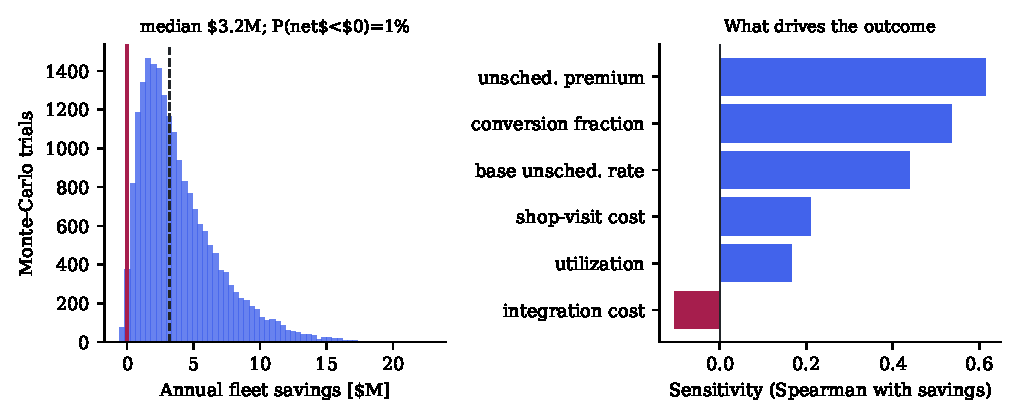
\includegraphics[width=\linewidth]{econ_impact}
    \end{column}
    \begin{column}{0.5\textwidth}
      100 CFM56-7B engines. The only monetized mechanism: less-biased prognosis
      converting \emph{unscheduled} removals into \emph{scheduled} ones.
      \medskip

      Median \alert{\$3\,M/year}, p10 \$0.9\,M, p90 \$8\,M, net-negative in
      $1\,\%$ of draws. \alert{Read the spread, not the median.}
      \medskip

      \textbf{Why it could be zero:} the isolation wall is unbroken; false alarms
      erode trust; the sim-to-real gap preserved the ranking but not the magnitude;
      mature operators already catch most failures --- and the absolute rate is anchored
      to the \emph{industry} band, not to our fleet's optimistic raw numbers.
    \end{column}
  \end{columns}
\end{frame}

% =========================================================================
\section{What to take away}
% =========================================================================

\begin{frame}[t]{The split verdict}
  \lead{Neither family wins outright, and the pattern is the useful part.}
  \begin{columns}[T]
    \begin{column}{0.48\textwidth}
      \textbf{\textcolor{bluec}{Learning wins}} where the task is
      \emph{statistical aggregation over time}:
      \begin{itemize}\small
        \item prognosis: $858$ vs $1981$ cycles ($\sim$2.3$\times$ over fielded practice,
          $\sim$1.3$\times$ over the best classical method), robust across architectures and
          sensor quality
        \item detection timing: $12\times$ earlier at equal false alarms
        \item calibrated uncertainty: $6\times$ tighter at honest coverage
      \end{itemize}
    \end{column}
    \begin{column}{0.48\textwidth}
      \textbf{\textcolor{redc}{Nobody wins}} where the task is bounded by
      \emph{what the sensors observed}:
      \begin{itemize}\small
        \item confusable isolation: $31\,\% = 31\,\%$
        \item the fix is $+77$ percentage points from \emph{real} station probes
        \item virtual sensors add exactly nothing
      \end{itemize}
    \end{column}
  \end{columns}
  \vspace{3mm}
  \begin{alertblock}{And physics did not lose --- it diagnosed the limits}
    The influence-matrix geometry predicted, \emph{before any learning ran}, where every
    method would fail. Injecting physics into the learner failed twice; using it to know the
    limits succeeded.
  \end{alertblock}
\end{frame}

\begin{frame}[t]{What an engineering organization should do on Monday}
  \lead{In order of how much money each moves.}
  \begin{enumerate}
    \item \textbf{Deploy learning for prognosis first.} The clear business case:
      maintenance slotting and lease planning, with calibrated intervals.
    \item \textbf{Detection: modern change detection with tuned windows.} The win
      came from window search --- cheap and auditable --- not from depth.
    \item \textbf{Isolation: buy sensors, not models.} And specifically probes at
      \emph{new stations}; quieter probes at the old ones do not help.
    \item \textbf{Redesign the report schedule before buying anything.} One
      procedural report condition recovers most of what deliberate spread offers.
    \item \textbf{Protect the sensor estate.} A drifting thermocouple corrupts
      every consumer downstream, learned or classical.
    \item \textbf{Distrust untuned comparisons in either direction} --- both
      families moved dramatically under the same budget; scoreboards inverted.
    \item \textbf{Demand pre-registration of vendor claims.} A split verdict is
      what honest evaluation looks like; a clean sweep should raise suspicion.
  \end{enumerate}
\end{frame}

\begin{frame}[t]{What transfers off this simulator --- and what does not}
  \lead{Stating this precisely is the price of using synthetic data.}
  \begin{columns}[T]
    \begin{column}{0.48\textwidth}
      \textbf{Transfers:} rankings, mechanisms and geometry. Which method wins
      where and why; the observability structure any CFM56-class cockpit set
      shares; the sensor-acquisition logic.
      \medskip

      Every operational claim in this work is of that kind.
    \end{column}
    \begin{column}{0.48\textwidth}
      \textbf{Does not transfer:} absolute performance numbers. An RMSE of $858$
      cycles is a property of this simulated world and its noise settings.
      \medskip

      \textbf{Honest limits:} synthetic and linearized world (audited to the noise
      floor); two snapshot conditions with scatter; EGT is a station-45 proxy;
      one compact architecture per task.
    \end{column}
  \end{columns}
  \vspace{4mm}
  \begin{block}{Reproducibility}
    The entire evidence base regenerates in \alert{about eleven minutes} on one
    desktop machine, GPU stages included. Every figure and number in the report
    and in these slides comes from a script --- none is copied by hand.
  \end{block}
\end{frame}

\begin{frame}[standout]
  The split verdict is the result.\\[4mm]
  {\normalsize A method comparison that produces a clean sweep\\
  is usually measuring effort, not method.}
\end{frame}

% =========================================================================
\appendix

\begin{frame}[t]{Appendix --- the pipeline}
  \centering
  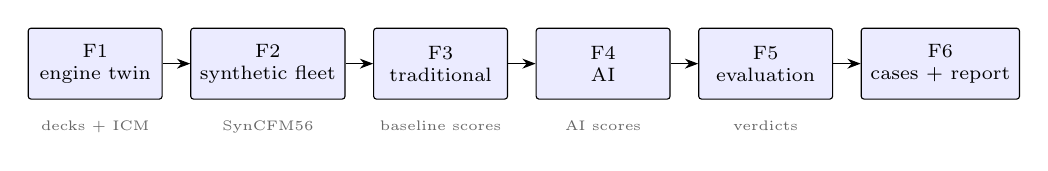
\begin{tikzpicture}[font=\scriptsize, node distance=3.5mm,
      ph/.style={draw, rounded corners=1pt, minimum height=9mm, minimum width=17mm,
                 align=center, fill=blue!8},
      gate/.style={font=\tiny, text=black!60}]
    \node[ph] (f1) {F1\\engine twin};
    \node[ph, right=of f1] (f2) {F2\\synthetic fleet};
    \node[ph, right=of f2] (f3) {F3\\traditional};
    \node[ph, right=of f3] (f4) {F4\\AI};
    \node[ph, right=of f4] (f5) {F5\\evaluation};
    \node[ph, right=of f5] (f6) {F6\\cases + report};
    \foreach \a/\b in {f1/f2, f2/f3, f3/f4, f4/f5, f5/f6}{
      \draw[-{Stealth}] (\a) -- (\b);}
    \node[gate, below=1.5mm of f1] {decks + ICM};
    \node[gate, below=1.5mm of f2] {SynCFM56};
    \node[gate, below=1.5mm of f3] {baseline scores};
    \node[gate, below=1.5mm of f4] {AI scores};
    \node[gate, below=1.5mm of f5] {verdicts};
  \end{tikzpicture}
  \vspace{4mm}

  {\small Each phase ends in a pass/fail gate with a criterion stated in advance.
  Extensions beyond F6 follow the same discipline: operating-point tomography,
  a ten-line limitation-overcoming programme, two ground-truth-validated
  certificates, and the economic study.}
\end{frame}

\begin{frame}[t]{Appendix --- the traditional detection stack}
  \centering
  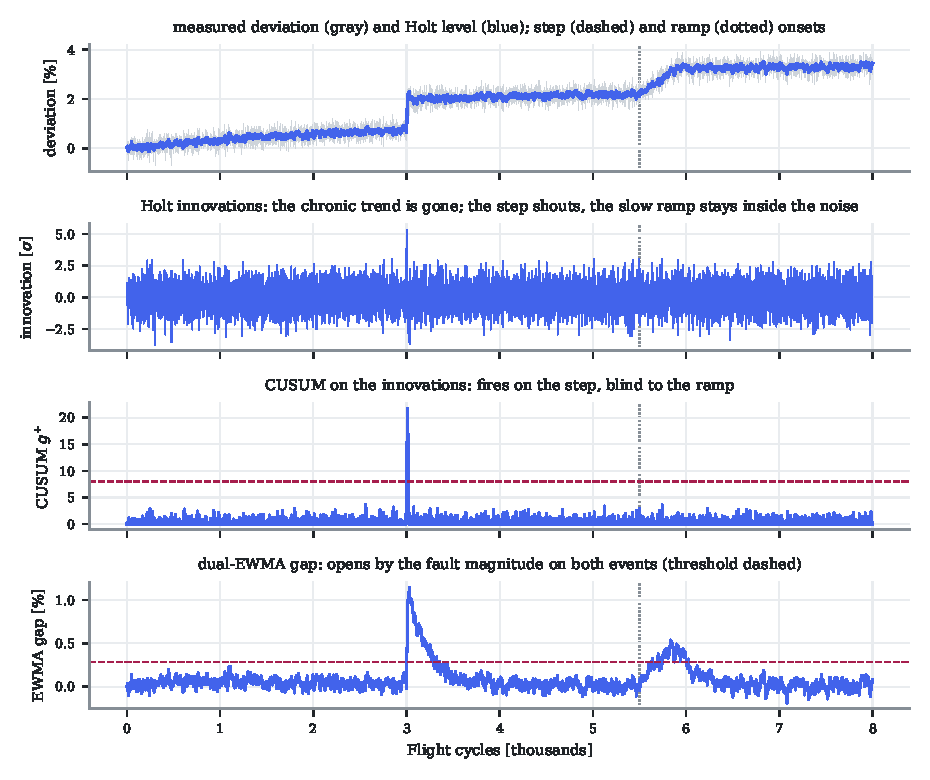
\includegraphics[width=0.56\textwidth]{detector_anatomy}\\[1mm]
  {\scriptsize Step detectors belong on \emph{innovations}: on raw deviations the chronic
  trend integrates without bound and alarms every engine. And a trend-shift detector cannot
  see acute ramps --- only the dual-EWMA gap does.}
\end{frame}

\begin{frame}[t]{Appendix --- is the geometry robust to calibration?}
  \centering
  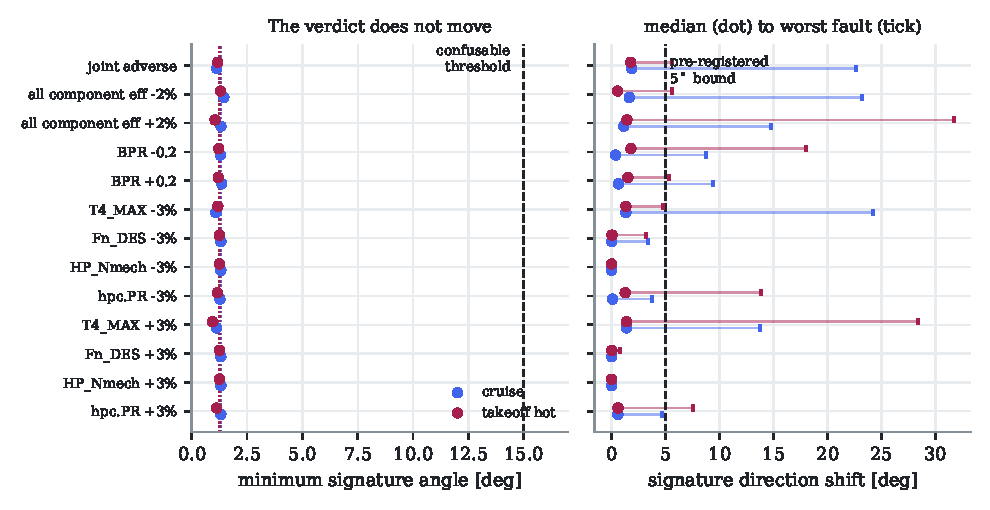
\includegraphics[width=0.85\textwidth]{icm_robustness}\\[1mm]
  {\scriptsize Every calibration knob perturbed inside its own contract
  tolerance. The verdict that matters is invariant: rank 3, minimum angle
  $0.94$--$1.45^{\circ}$, same most-confusable pair every time. What is
  \emph{not} invariant is the exact membership of the confusable list at its
  $15^{\circ}$ boundary --- the weakest columns are near-null vectors, and a
  near-null vector has no stable direction.}
\end{frame}

\begin{frame}[t]{Appendix --- the compute budget}
  \centering{\tiny% AUTOGENERATED by scripts/make_report_assets.py — do NOT edit by hand
% machine: Apple M5, 10 cores, 16 GB, torch 2.12.1 (mps)
\begin{tabular}{llcr}
\toprule
Stage & Script & Device & Wall time [s] \\
\midrule
  design point & \code{scripts/run_design_point.py} & CPU & 2 \\
  sls anchors & \code{scripts/run_anchors.py} & CPU & 13 \\
  baseline decks & \code{scripts/make_decks.py} & CPU & 214 \\
  corrected baseline & \code{scripts/make_corrected_baseline.py} & CPU & 1 \\
  icm grid & \code{scripts/make_icm.py} & CPU & 71 \\
  fleet generation & \code{scripts/make_fleet.py} & CPU & 40 \\
  audit dataset & \code{scripts/audit_dataset.py} & CPU & 12 \\
  audit nonlinearity & \code{scripts/audit_nonlinearity.py} & CPU & 20 \\
  traditional pipeline & \code{scripts/run_trad.py} & CPU & 106 \\
  ai suite & \code{scripts/run_ai.py} & CPU+GPU & 27 \\
  hybrid ablation & \code{scripts/run_hybrid.py} & CPU+GPU & 104 \\
  pcs & \code{scripts/run_pcs.py} & CPU+GPU & 46 \\
  \midrule
  \textbf{Full pipeline} & & & \textbf{657} \\
\bottomrule
\end{tabular}
}
  \vspace{3mm}

  {\scriptsize Reference machine: an Apple M5 desktop chip, 10 cores, 16\,GB, tensor
  training on its GPU through the torch MPS backend --- consumer hardware, deliberately.
  If it only ran on a cluster, it would not be adoptable.}
\end{frame}

\end{document}
